\subsection{Settings}
\begin{frame}[noframenumbering]{Table of Contents}
  \tableofcontents[currentsection, currentsubsection]
\end{frame}


\begin{frame}
  Let $\Omega = (-1,1)^2$. Define $f\in H^1_0(\Omega)$ by 
  $f(x)=\tilde{f}(|x|)$ for all $x\in\Omega$ with
  \begin{align*}
    \tilde{f}(r)\coloneqq 
    \begin{cases}
      \alpha-12(2-9r) & \text{if } 0\leq r\leq\frac{1}{6},\\
      6r\alpha-\frac{1}{r} & \text{if } \frac{1}{6}\leq r\leq
      \frac{1}{3}\\
      2\alpha+6\pi\sin(\pi(6r-2))-\frac{1}{r}\cos(\pi(6r-2)) &
      \text{if } \frac{1}{3}\leq r\leq\frac{1}{2},\\
      \alpha(5-6r)+\frac{1}{r}&
      \text{if } \frac{1}{2}\leq r\leq\frac{5}{6},\\
      -3\pi\sin(\pi(6r-5))+\frac{1+\cos(\pi(6r-5))}{2r} &
      \text{if } \frac{5}{6}\leq r\leq 1.
    \end{cases}
  \end{align*}
  
  \begin{figure}[!ht]
    \centering
    \begin{subfigure}{.4\linewidth}
      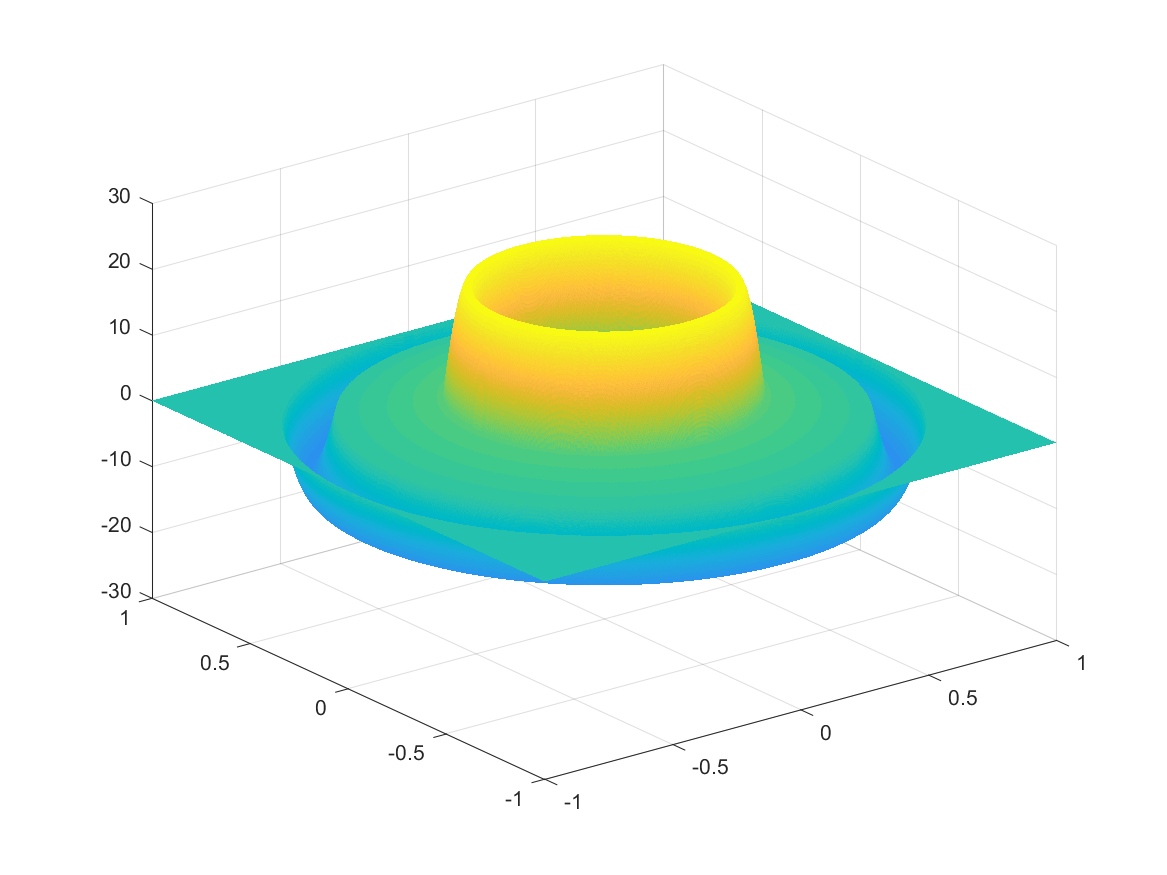
\includegraphics[width=\linewidth]
        {pictures/experiments/settings/f01/rhs.png}
      \caption*{$f$ for $\alpha=1$}
    \end{subfigure}
    \quad
    \begin{subfigure}{.4\linewidth}
      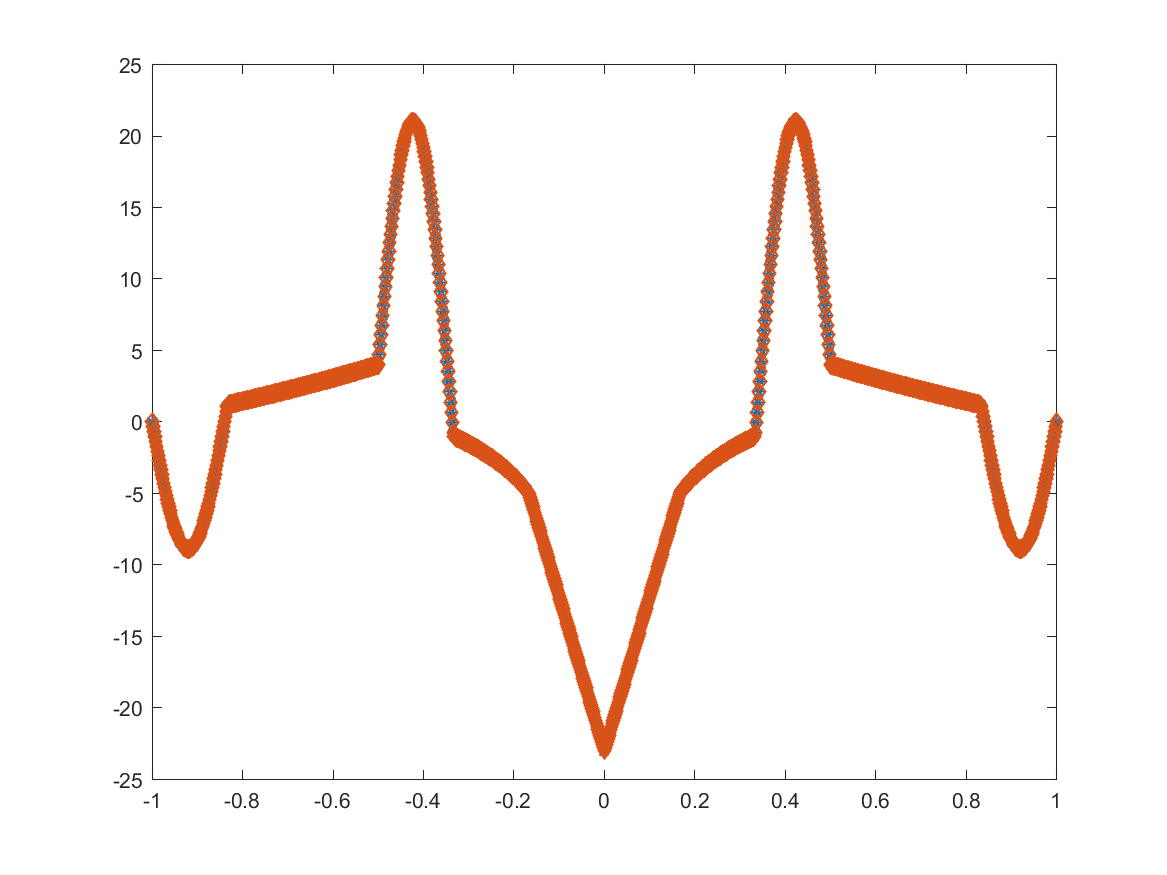
\includegraphics[width=\linewidth]
        {pictures/experiments/settings/f01/rhsAxis.png}
      \caption*{$f$ for $\alpha=1$ along the axes}
    \end{subfigure}
  \end{figure}
\end{frame}

\begin{frame}
  Then the solution to the continuous problem with input signal $f$ is given by
  $u\in H^1_0(\Omega)$ defined by $u(x)=\tilde{u}(|x|)$ for all $x\in\Omega$
  with 
  \begin{align*}
    \tilde{u}(r)\coloneqq
    \begin{cases}
      1 & \text{if } 0\leq r\leq\frac{1}{6},\\
      6r & \text{if } \frac{1}{6}\leq r\leq\frac{1}{3},\\
      2 &\text{if } \frac{1}{3}\leq r\leq\frac{1}{2},\\
      5-6r &\text{if } \frac{1}{2}\leq r\leq\frac{5}{6},\\
      0 &\text{if } \frac{5}{6}\leq r.
    \end{cases}
  \end{align*}
  
  \begin{figure}[!ht]
    \centering
    \begin{subfigure}{.4\linewidth}
      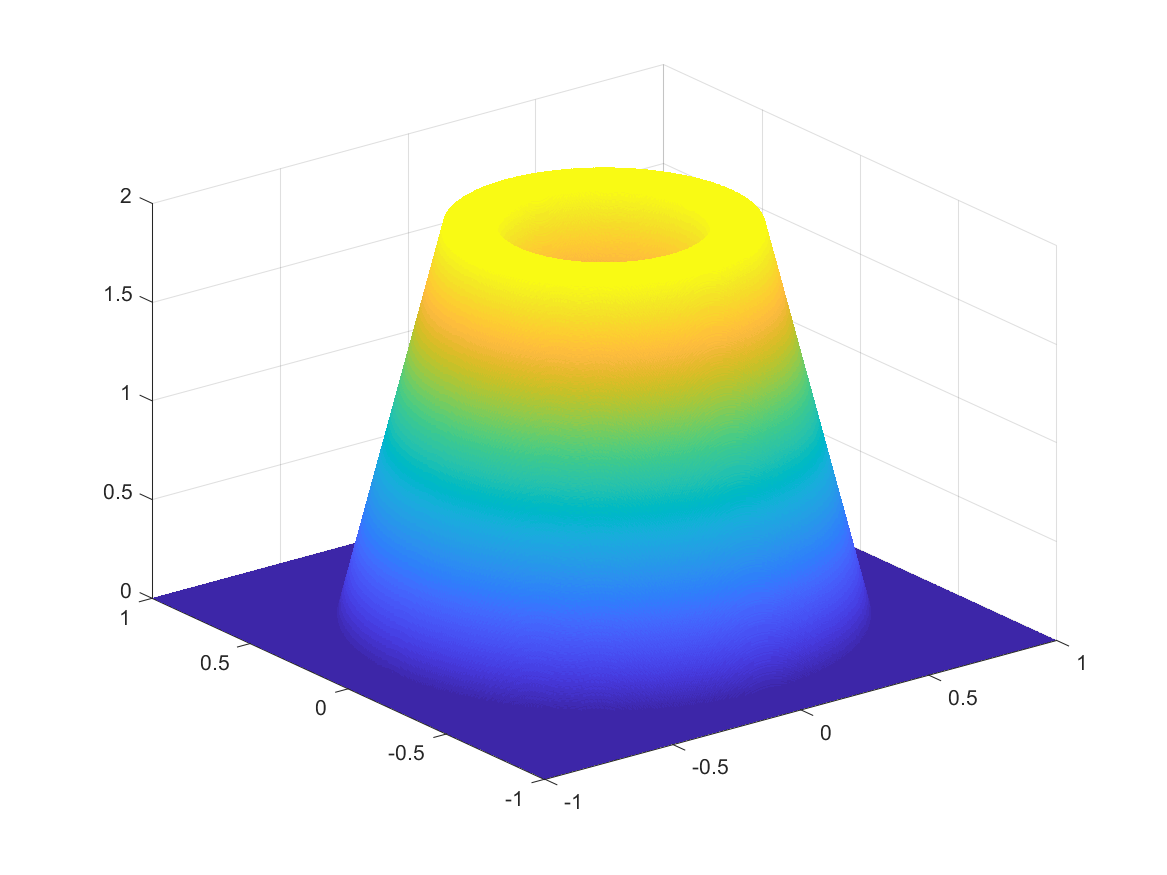
\includegraphics[width=\linewidth]
        {pictures/experiments/settings/f01/exactSolution.png}
      \caption*{$u$}
    \end{subfigure}
    \quad
    \begin{subfigure}{.4\linewidth}
      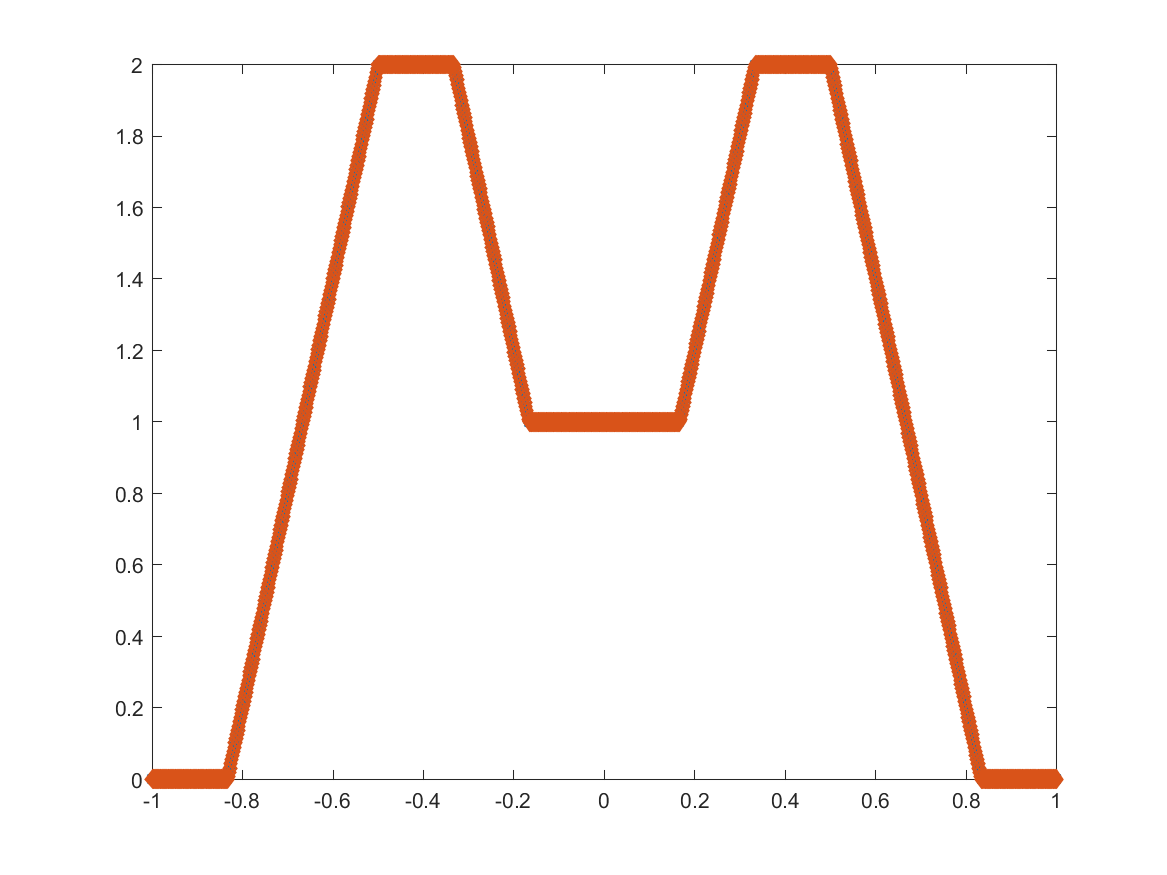
\includegraphics[width=\linewidth]
        {pictures/experiments/settings/f01/exactSolutionAxis.png}
      \caption*{$u$ along the axes}
    \end{subfigure}
  \end{figure}

  \pause
  It holds $E(u)\approx -2.058034062391$.
\end{frame}


\begin{frame}
  For $\alpha = 10000$ let the input signal represent the grayscale of an image
  in $[0,1]^{256\times 256}$ multiplied with $\alpha$ scaled to the domain
  $\Omega=(0,1)^2$.

  \begin{figure}[!ht]
    \centering
    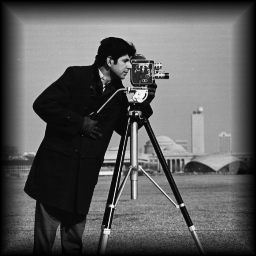
\includegraphics[width=.5\linewidth]
      {pictures/experiments/settings/images/f2bcameraman.png}
    \caption*{Image cameraman}
  \end{figure}
\end{frame}

\begin{frame}{Initial Triangulations for the Input Signals}
  \begin{figure}[!ht]
    \centering
    \begin{subfigure}{.45\linewidth}
      \caption*{Input signal $f$}
      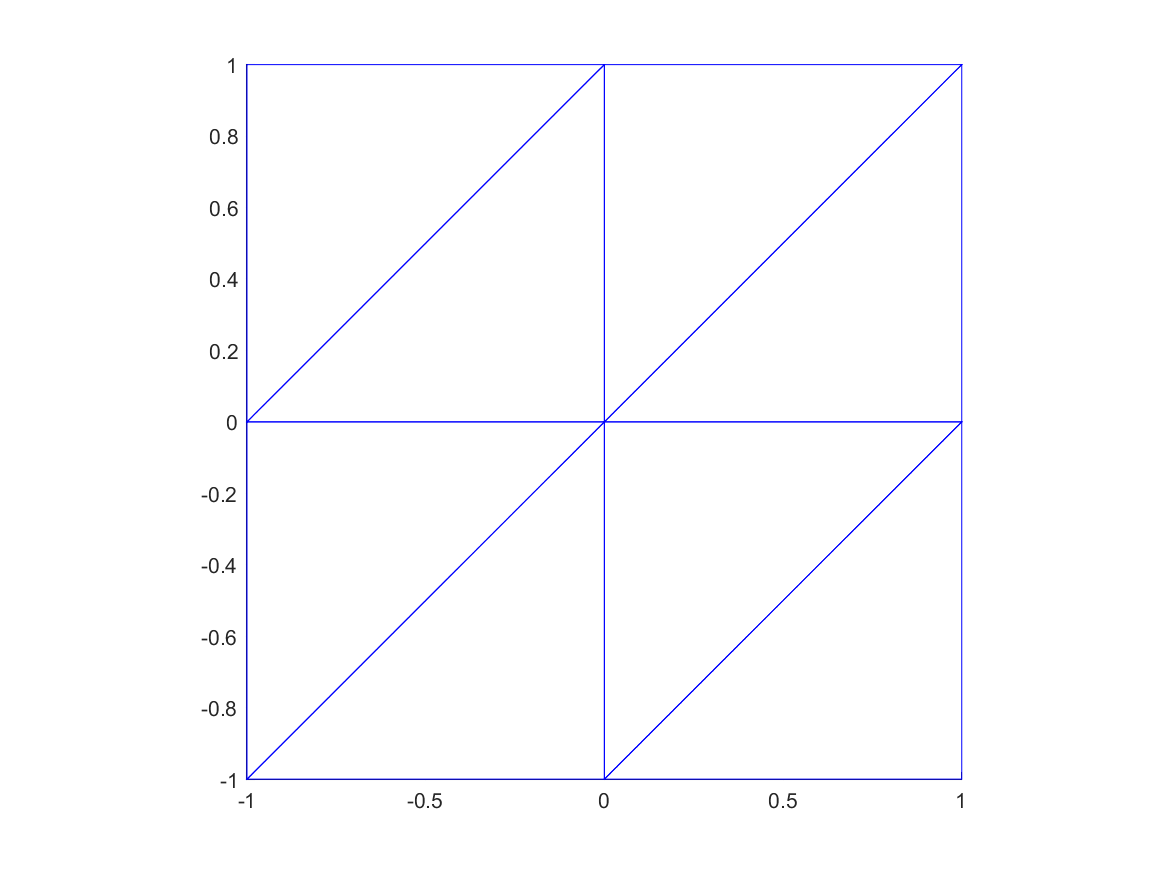
\includegraphics[width=\linewidth]
        {pictures/experiments/settings/f01/triangulation.png}
      \caption*{$\Omega = (-1,1)^2$}
    \end{subfigure}
    \begin{subfigure}{.45\linewidth}
      \caption*{Input signal cameraman}
      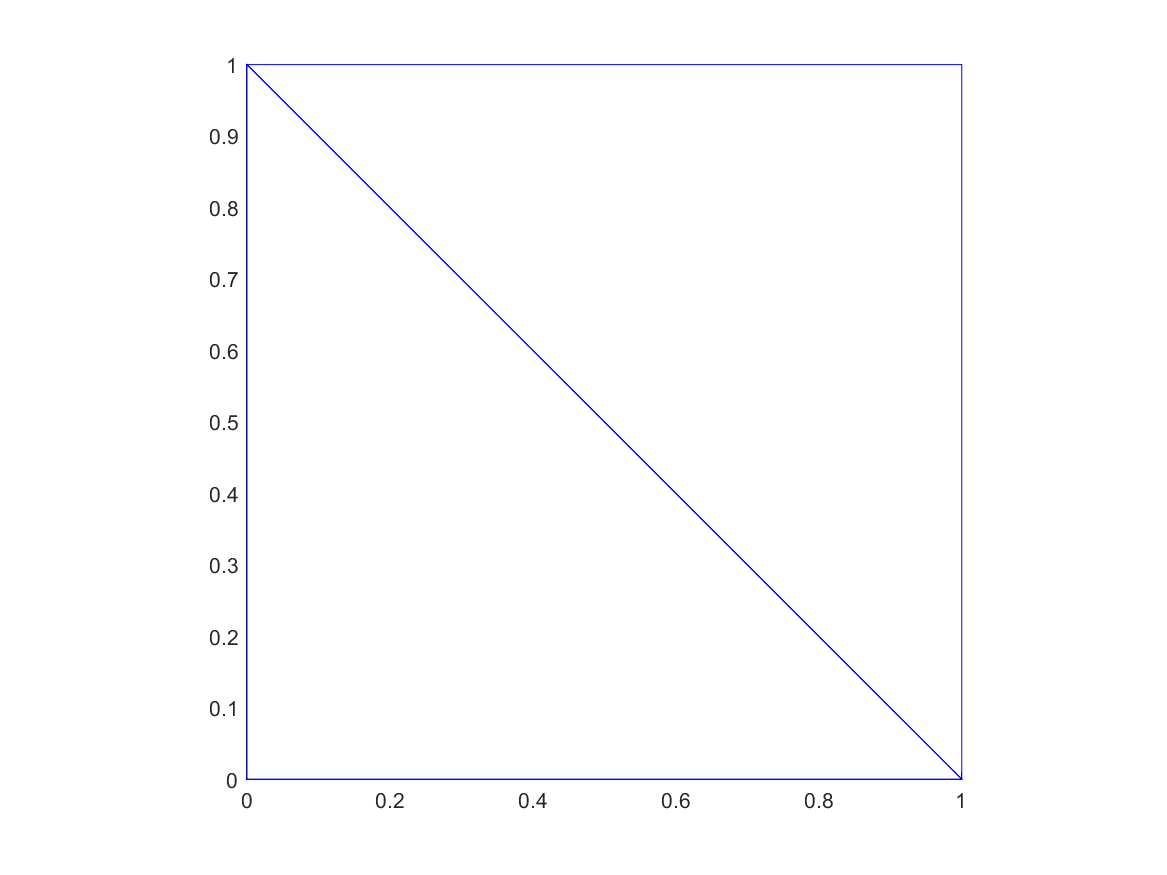
\includegraphics[width=\linewidth]
        {pictures/experiments/settings/images/triangulation.png}
      \caption*{$\Omega = (0,1)^2$}
    \end{subfigure}
  \end{figure}
\end{frame}

\subsection{Choice of Parameters}
\begin{frame}[noframenumbering]{Table of Contents}
  \tableofcontents[currentsection, currentsubsection]
\end{frame}

\begin{frame}{Choice of $\tau$}
  For the rest of the presentation (unless otherwise specified) let the bulk
  parameter be $\theta = 0.5$, and $\varepsilon_\textup{stop}= 10^{-4}$.
  \only<1>{
  \begin{figure}[!ht]
    \centering
    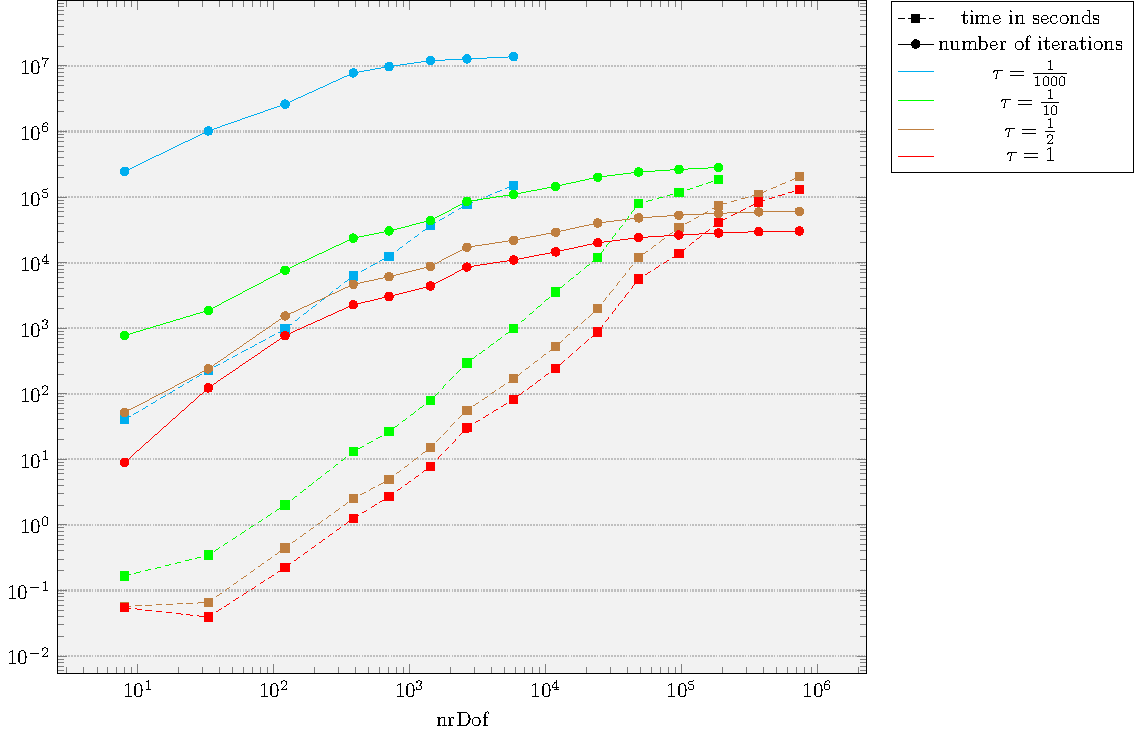
\includegraphics[width=0.9\linewidth]
      {pictures/experiments/choiceOfParameters/tau/miscF.pdf}
    \caption*{Input signal $f$}
  \end{figure}}
  \only<2>{
  \begin{figure}[!ht]
      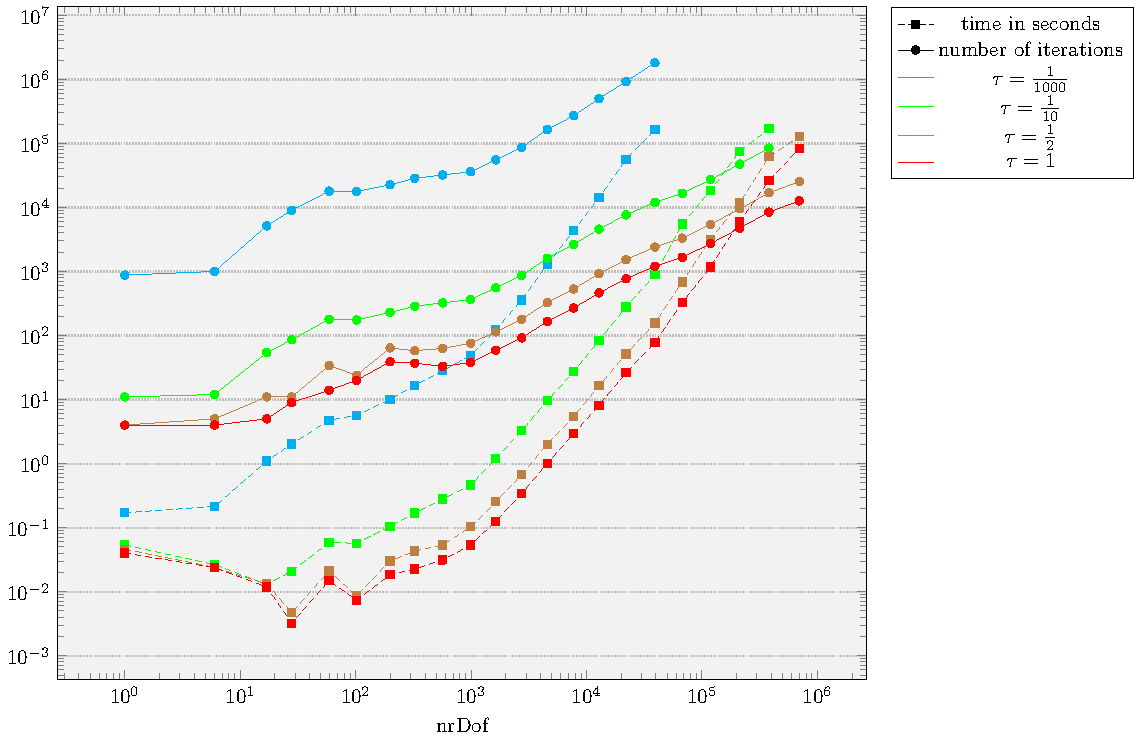
\includegraphics[width=0.9\linewidth]
        {pictures/experiments/choiceOfParameters/tau/miscCam.pdf}
      \caption*{Input signal camerman}
  \end{figure}}
  \only<3>{
  \begin{figure}[!ht]
      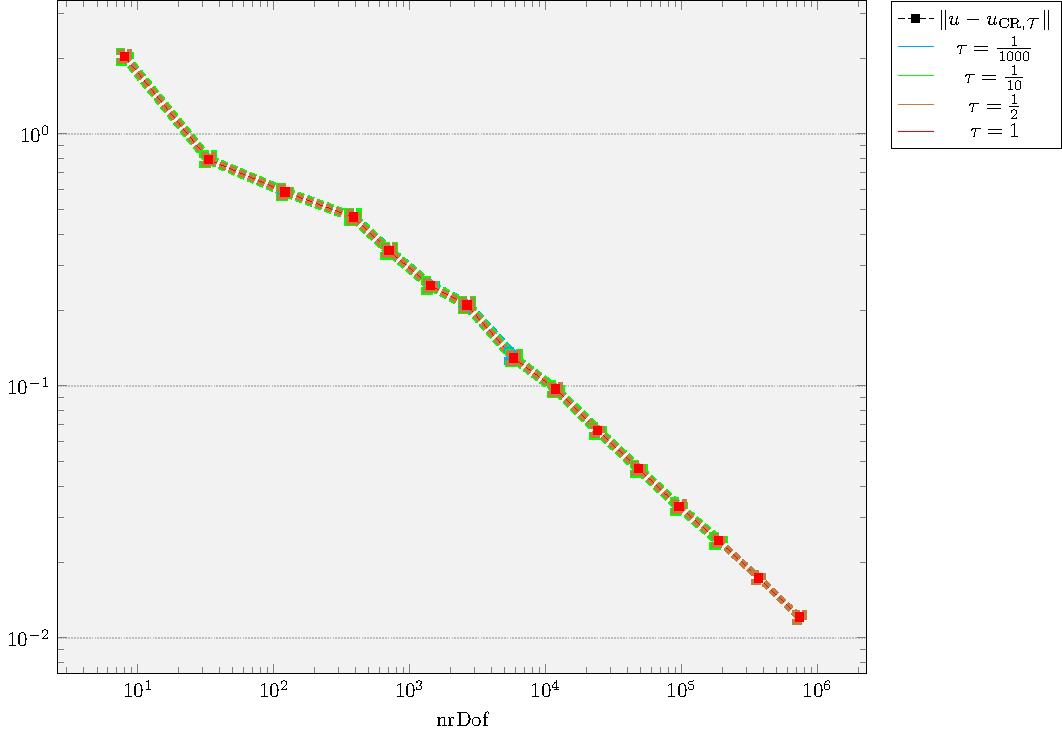
\includegraphics[width=0.8\linewidth]
        {pictures/experiments/choiceOfParameters/tau/convergenceF.pdf}
      \caption*{Input signal $f$}
  \end{figure}}
\end{frame}

\begin{frame}{Conclusion and Hypothesis}
  For the rest of the presentation $\tau = 1$.

  \pause
  \medskip
  
  Convergence of the iterates of the primal-dual iteration to the discrete
  solution $\ucr$ followed from
  \begin{align*}
    \sum_{j=1}^\infty\Vert \ucr-u_j\Vert^2 
    \leq
    \frac{1}{2\alpha{\color<3>{red}{\tau}}}
    \left({\color<5->{red}{\vvvert \ucr-u_0\vvvert^2_\nc}}
    + \Vert \bar\Lambda_0-\Lambda_0\Vert^2\right).
  \end{align*}

  \pause
  \pause
  Settings with $\tau = 1.2$ and no convergence were observed.
  \pause
  \pause

  \medskip
  For $\vcr\in\CR^1_0(\Tcal)$, define $J_1:\CR^1_0(\Tcal)\to P_1(\Tcal)\cap
  C_0(\Omega)$ by
  \begin{align*}
    J_1\vcr(z)\coloneqq |\Tcal(z)|^{-1}\sum_{T\in\Tcal(z)}\vcr|_T(z)
    \quad\text{for all }z\in\Ncal(\Omega).
  \end{align*}

  \pause

  Use $\hat u_0 \coloneqq J_1 u_{\textup{CR},\Tcal}\in P_1(\Tcal)\cap
  C_0(\Omega)\subseteq P_1\big(\hat\Tcal\big)\cap C_0(\Omega)
  \subseteq \CR^1_0\big(\hat\Tcal\big)$ as input for the iteration on the
  refined triangulation $\hat\Tcal$.
\end{frame}

\begin{frame}{Choice of $\varepsilon_\textup{stop}$}
  With $\tau=1$ the stopping criterion reads $\vvvert u_j-u_{j-1}\vvvert_\nc<
  \varepsilon_\textup{stop}.$
  \begin{figure}[!ht]
    \centering
    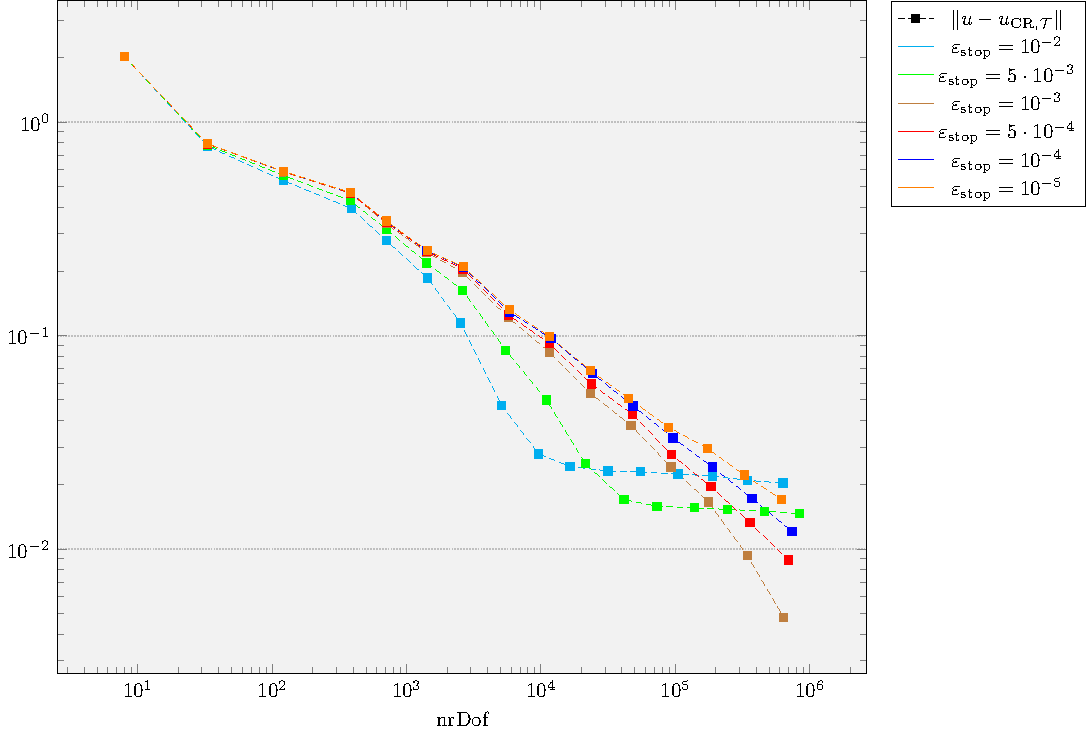
\includegraphics[width=0.8\linewidth]
      {pictures/experiments/choiceOfParameters/epsStop/convergence.pdf}
  \end{figure}

  \pause
  For the rest of the presentation $\varepsilon_\textup{stop} = 10^{-4}$.
  %$\vvvert\bullet\vvvert_\nc \approx h^{-1}\Vert\bullet\Vert$.
\end{frame}


\subsection{Guaranteed lower Energy Bound and Refinement Indicator}
\begin{frame}[noframenumbering]{Table of Contents}
  \tableofcontents[currentsection, currentsubsection]
\end{frame}

\begin{frame}
  TODO translate and rewrite
  \begin{theorem}
    \label{thm:gleb}
    Sei $\Omega$ konvex, $f\in H^1_0(\Omega)$ das Eingangssignal für
    mit Lösung $u\in H^1_0(\Omega)$ und minimaler
    Energie $E(u)$ sowie für  mit Lösung $\ucr\in
    \CR^1_0(\Omega)$ und minimaler Energie $\Enc(\ucr)$.
    Dann gilt
    \begin{align*}
      \Enc(\ucr)+\frac{\alpha}{2}\Vert u-\ucr\Vert^2
      -\frac{\kappa_\CR}{\alpha}\Vert
      h_\Tcal(f-\alpha\ucr)\Vert \Vert\nabla f\Vert\leq E(u).
    \end{align*}
    Dabei ist die Konstante $\kappa_\CR\coloneqq\sqrt{1/48+1/j_{1,1}^2}$ mit der
    kleinsten positiven Nullstelle $j_{1,1}$ der Bessel-Funktion erster Art.
    Insbesondere gilt dann für 
    \begin{align}
      \label{eq:gleb}
      \Egleb 
      \coloneqq 
      \Enc(\ucr) - \frac{\kappa_\CR}{\alpha}\Vert h_\Tcal(f-\alpha\ucr)\Vert
      \Vert \nabla f\Vert,
    \end{align}
      dass $\Enc(\ucr)\geq \Egleb$ und $E(u)\geq \Egleb$.
  \end{theorem}
\end{frame}


\begin{frame}
  TODO translate and rewrite, leave out the $d$ and make it 2. Say we choose
  $\gamma=1$ because we want to refine towards the discontinuities

  \begin{definition}[Verfeinerungsindikator]
    Für $d\in\mathbb{N}$ (in dieser Arbeit stets $d=2$) und $0<\gamma\leq 1$
    definieren wir für alle $T\in\Tcal$ und $\ucr\in\CR^1_0(\Tcal)$ die
    Funktionen
    \begin{align*}
      \eta_\text{V}(T)
      &\coloneqq
      |T|^{2/d}\Vert f-\alpha \ucr\Vert^2_{L^2(T)}\quad\text{und }\\
      \eta_\text{J}(T)
      &\coloneqq
      |T|^{\gamma/d}\sum_{F\in\Ecal(T)}\left\Vert [\ucr]_F\right\Vert_{L^1(F)}.
    \end{align*} 
    Damit definieren wir den Verfeinerungsindikator
    $\eta\coloneqq\sum_{T\in\Tcal}\eta(T)$, wobei
    \begin{align*} 
      \eta (T)
      \coloneqq
      \eta_\text{V}(T) + \eta_\text{J}(T)\quad\text{für alle } T\in\Tcal.
    \end{align*} 
  \end{definition}
\end{frame}

\begin{frame}
  cameraman triangulation figures to show the effect of the refinement 
  indicator
\end{frame}

\begin{frame}
  convergence graphs error and refinement indicator and probably its volume
  and jump contributions

  adaptive and uniform

  maybe also plot refinement indicator and its contributions for cameraman

  say expected rates from bartels and compare to them
\end{frame}


\begin{frame}
  plot differences between energies and gleb 

  plot the differences between the discrete energies and the exact energy
  energy in the graph with all gleb differences

  note that Enc -Egleb and E - Egleb dont differ much obviously because
  Enc - E tends to zero (as seen in the plots)

  show strict convecity theorem here to show that it holds (even 'better' than
  the theorem guarantees)
\end{frame}

\begin{frame}
  show error, eta (without contributions) together with the differences
  of the energies and EGLEB
\end{frame}

\subsection{Convergence of the Iteration} \begin{frame}[noframenumbering]{Table of Contents}
  \tableofcontents[currentsection, currentsubsection]
\end{frame}

\begin{frame}{TODO}

  think about where to position this topic wise

  \begin{figure}[!ht]
    \centering
    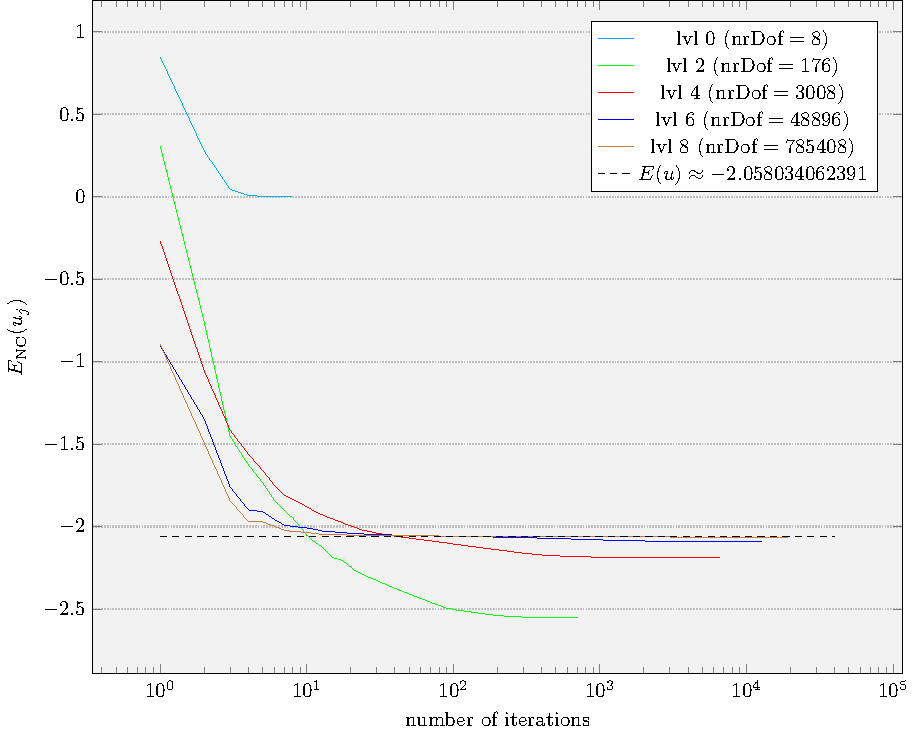
\includegraphics[width=0.8\linewidth]
      {pictures/experiments/convergenceIteration/convergenceIteration.pdf}
  \end{figure}

\end{frame}

\begin{frame}
  previous frame cont.

  show that the energy converges from above to the exact energy (not
  necessarily monotonly, i.e. choose some example where it simply converges
  and one example where there are oscillations, i.e. two pictures here

  also mention that it converges to something slightly below the exact energy,
  i.e. choose the pictures accordingly, maybe even plot the error between
  the energies of the iterates and the exact energy

  THAT MEANS choose one picture from $f$ where the exact energy can be seen 
  and maybe one from the cameraman

  mention that during the afem loop we will see, that this undershooting 
  decrease (as one would expect, the discrete energy converges to the exact
  energy)
\end{frame}

\begin{frame}
  show the result of an iteration (plot of uApprox next to uExact) 
  (along the axes as well)
  and show cameraman grayscale plot

  definitely mention degrees of freedom if only one level is shown!!!
\end{frame}
